\documentclass[a4paper,12pt]{report}
\usepackage[T1]{fontenc}
\usepackage[polish]{babel}
\usepackage[utf8]{inputenc}
\usepackage{amsmath}
\usepackage{graphicx}

\title{Notatki z wykładu ,,Nieskończone Alfabety''}
% jeśli rozwijasz ten dokument, dopisz się do listy autorów
% porządek autorów powinien być alfabetyczny
\author{Tomasz Wysocki}
\begin{document}
\maketitle
\newpage
\tableofcontents
\newpage
\chapter {Wykład I: wstęp do nieskończonych alfabetów}
\section {Dlaczego warto badać nieskończone alfabety?}
\section {Znane modele automatów dla słów}

Większość wykładu dotycząca nieskończonych alfabetów będzie poświęcona modelom operującym na słowach. Decyzja taka wynika z faktu, że problemy dotyczące operacji na drzewach nie wpisują się w tematykę tego przedmiotu.

Przez większość wykładu prezentowane modele będą rozważały jedynie równość elementów z nieskończonego alfabetu. Alfabet nie musi mieć zatem żadnej narzuconej struktury.

Def. niech A będzie skończonym zbiorem ,,etykiet'', D - nieskończonym zbiorem danych. Wtedy strukturę $w \in (A x D)^*$ nazywamy ,,słowem z danymi''.

Większość automatów używanych w trakcie wykładu, będzie operować na słowach w postaci zdefiniowanej powyżej.

\subsection{Przykłady}
\begin{figure}
\begin{center}
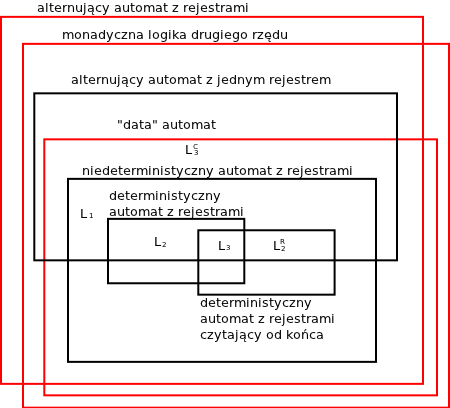
\includegraphics{images/podzial_automatow.png}
\end{center}
\caption{Moc wyrazu poszczególnych modeli}
\end{figure}
Na potrzeby przykładów przyjmujemy, że $ w \in D^* $

$L_1$ = ,,pierwsza litera jest taka sama jak ostatnia litera''

$L_1 = {\bigcup \limits _{d \in D} dD^*d + d}$

$L_2$ = ,,pierwsza litera pojawia się ponownie''

$L_2 = {\bigcup \limits _{d \in D} dD^*dD^*}$

$L_3$ = ,,jakaś litera pojawia się dwukrotnie''

$L_3 = {\bigcup \limits _{d \in D} D^*dD^*dD^*}$

\section {Definicja niedeterministycznego automatu z rejestrami}
Niedeterministyczny automat z rejestrami jest zadawany przez:
\begin{itemize}
\item skończony zbiór etykiet A
\item skończony zbiór stanów Q
\item stany początkowe i końcowe $I,F \in Q$
\item skończony zbiór nazw rejestrów R
\item relację zadającą przejścia automatu $\delta 
\in Q x A x 2^R x Q x (R \cup \bot)$
\end{itemize}

Konfiguracją automatu jest $(q,r) \in Q x (R \rightharpoondown D)$.

\paragraph {Należenie krotki $(q,a,r_1,r_3,p,r_4)$ do relacji przejścia automatu, należy rozumieć jako:} automat będąc w stanie q i czytając etykietę a oraz daną, która jest równa z rejestrami $r_1,r_3$ i nierówna z pozostałymi rejestrami, przechodzi do stanu p i zapisuje czytaną daną do rejestru $r_4$.
\end{document}